\section{Class diagram}
In this section, the class diagram of the dynamic Bayesian network, see \figref{figure:class-diagram}, will be shown and explained, to give an overview of the structure of the Bayesian network implementation.

\begin{figure}[H]
     \centering
     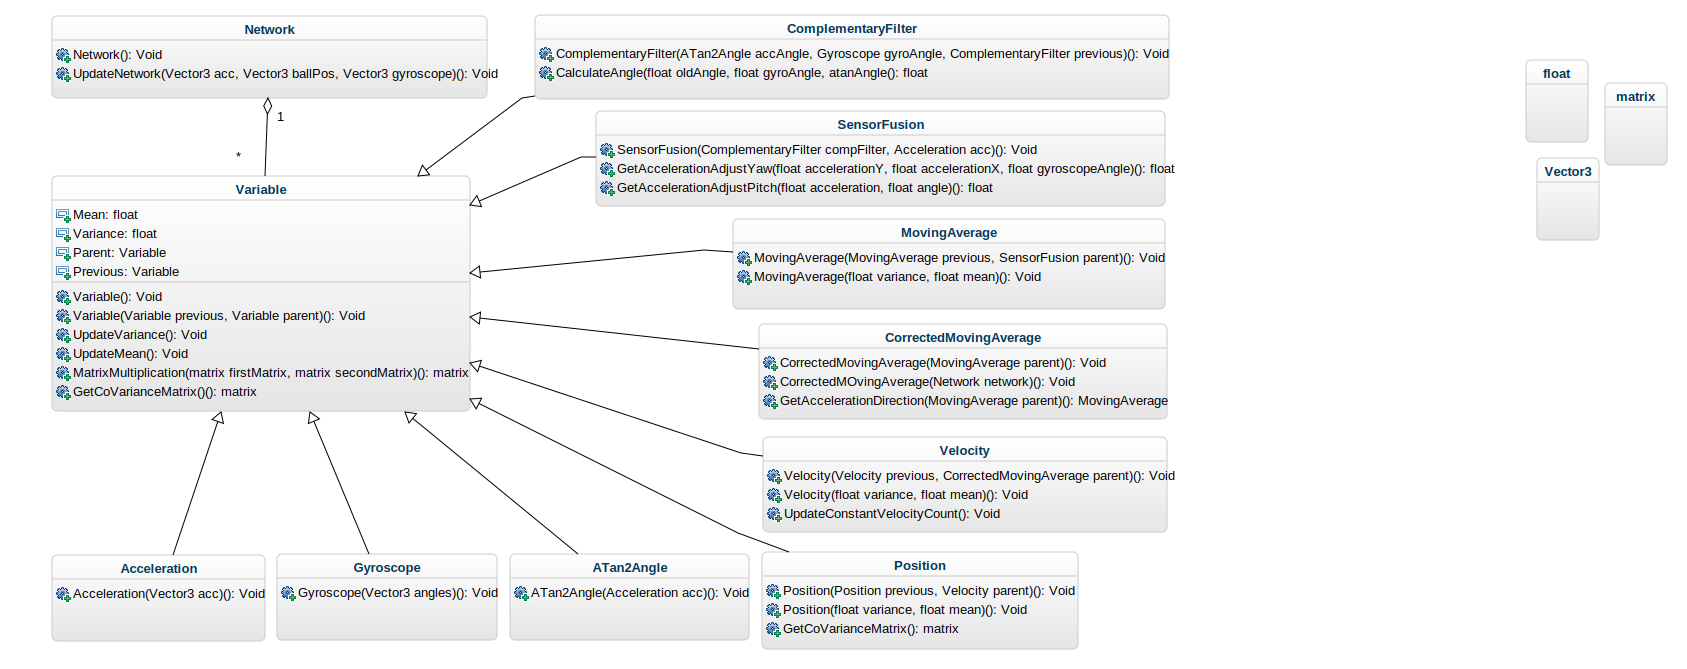
\includegraphics[trim=0cm 0cm 5cm 0cm,clip,scale=1.25]{implementation/classdiagramb}
     \caption{Class diagram for developed navigation library.}     
     \label{figure:class-diagram}
\end{figure}

To implement a dynamic Bayesian network, the structure from \figref{figure:class-diagram} was used.
The \textit{Network} class keeps track of the overall structure of the dynamic Bayesian network.
In order to keep track of the structure, the \textit{Variable} class has nine subclasses.
The Variable class exists to calculate the marginal probability distribution for each of its subclasses.
Each subclass then calculates the concrete probability distribution and constraints, which varies for each of the subclasses.

Concrete implementation of a sample of the classes in \figref{figure:class-diagram} will be described in the next sections.